\documentclass[10pt,a4paper,twocolumn]{article}
\usepackage[T1]{fontenc}
\usepackage[utf8]{inputenc}
\usepackage{lmodern,microtype}
\usepackage[margin=16mm,columnsep=6mm]{geometry}
\usepackage{amsmath,booktabs,tabularx,array}
\usepackage{graphicx,xcolor,tikz,pgfplots,balance}
\usepackage[font=small,labelfont=bf,skip=4pt]{caption}
\usepackage{titlesec,indentfirst}
\usepackage[hidelinks]{hyperref}
\pgfplotsset{compat=1.18}
\usepgfplotslibrary{groupplots,fillbetween}
\definecolor{blue}{HTML}{245581}
\definecolor{orange}{HTML}{BD5B21}
\definecolor{teal}{HTML}{187E78}
\titleformat{\section}{\normalsize\bfseries}{\thesection.}{.4em}{}
\titleformat{\subsection}{\small\bfseries}{\thesubsection}{.4em}{}
\titlespacing{\section}{0pt}{8pt}{4pt}
\titlespacing{\subsection}{0pt}{6pt}{3pt}
\setlength{\parindent}{1em}
\setlength{\parskip}{0pt}
\setlength{\textfloatsep}{8pt plus 2pt minus 2pt}
\setlength{\floatsep}{7pt plus 2pt minus 2pt}
\setlength{\intextsep}{7pt plus 2pt minus 2pt}
\renewcommand{\topfraction}{.95}
\renewcommand{\bottomfraction}{.85}
\renewcommand{\textfraction}{.05}
\renewcommand{\floatpagefraction}{.8}
\setcounter{topnumber}{4}
\setcounter{bottomnumber}{4}
\setcounter{totalnumber}{8}
\title{\vspace{-8mm}\Large\bfseries Brazil in a Global Atlas of Lyrical Themes:\\Chart Repertoires and Social Context}
\author{}
\date{\vspace{-10mm}\small Data freeze: 11 October 2026}
\begin{document}
\raggedbottom
\maketitle
\begin{abstract}
We compare lyrical themes across 68 music markets, with Brazil as a focal case. An archive of 47.43 million source records supports an intended geographical corpus of 153,501 recording IDs, all successfully classified. In the same 55 markets from 2017 to 2021, materialism, crime and weapons gained chart share, while romance remained common. Brazil had the largest increase in casual-sex themes. These patterns depend on how music is counted: romance represented 40.9\% of songs but 48.3\% of observed chart streams in the 51-market Top-200 panel. Genre and release-group comparisons show how changes in the songs entering charts can shape apparent cultural trends. We examine three focused relationships with inequality, gender conditions and homicide, accounting for measured repertoire and economic differences. A multilingual search comparison tests the sensitivity of the English search specification. The study provides a reproducible atlas of lyrics and chart exposure, while distinguishing these measures from residents' beliefs or behavior. Independent human accuracy estimates remain unavailable.
\end{abstract}

\section{Research question}
How do sexual, romantic, gender, material, and crime and conflict themes differ across music markets, and how do they relate to chart dynamics and external indicators? Brazil is a focal case, compared with other markets using the same measures. The analysis separates sexual content from objectification and misogyny, and thematic presence from endorsement. This allows several aspects of a song to coexist without collapsing them into one moral score.

The study combines historical charts, lyrics, Gemini classification and social indicators matched by year. A recording ID is the stable identifier linking a recording across sources and dates. A source record is one stored entry, so repeated chart appearances can create many records for the same song. A specialist check was reported by the project lead. Independent measurements of accuracy are still needed. We examine the songs circulating in each market, changes over time and associations with social conditions. A market identifies where a recording appears in the charts, rather than the artist's nationality or the listener's identity.

Six axes organize the analysis: \textbf{intimacy} (romance, heartbreak, reciprocity and sexual relations); \textbf{gender and power} (agency, objectification and misogyny); \textbf{status and inequality} (money, materialism and wealth); \textbf{violence and security} (crime, weapons and drugs); \textbf{digital environment} (access, search and connectivity). And \textbf{cultural circulation} (identity, genres and chart persistence). Brazil is the focal case. The atlas lets every market inspect its own profile, position and coverage.

\section{Related research and contribution}
Research on lyrics has already documented long-term changes in popular music. Brand, Acerbi and Mesoudi studied emotional expression over five decades of song lyrics, showing how popular songs can be used to examine cultural transmission and emotional change~\cite{brand}. Their emotional measures do not by themselves distinguish romance, sexual content, wealth, weapons or the stance taken toward violence. Our study makes those distinctions explicit and compares their circulation across markets.

Varnum and colleagues analyzed 14,661 songs in US charts between 1958 and 2016. They linked simpler lyrics to a larger supply of new songs and to chart success~\cite{varnum}. Parada-Cabaleiro and colleagues examined changes in lyrical complexity, repetition and emotional language across genres~\cite{parada}. Together, these studies show why an aggregate change in lyrics needs to be examined alongside the supply and type of songs entering the charts. We address that issue through genre and release-group decompositions, while recognizing that broad artist-derived tags and incomplete dates cannot fully explain repertoire selection.

International listening also varies with cultural and social context. Liu, Hu and Schedl studied cross-country music preferences in relation to culture, socioeconomic conditions and friendship~\cite{liu}. Schedl and colleagues identified country archetypes from listening patterns and used them in music recommendation~\cite{schedl}. Those studies motivate regional comparisons, but listening-pattern clusters and clusters of lyrical themes measure different things. A country can share themes with another without sharing the same songs or listeners.

The added contribution is a common 26-dimension lyrical taxonomy linked to recording IDs, circulation markets, years, chart days, recorded streams and dated social indicators. It separates romantic affection, sexual explicitness, gender representation and material or violent themes instead of combining them into one score. It also compares counting songs with counting chart exposure, and tests how much temporal change is associated with genre and release-group composition. This is a descriptive extension of earlier work, not evidence that chart lyrics directly measure national values. Its stronger multilingual claims require the independent human validation described below.


\section{Corpus and method}
\subsection{Sources, units, and coverage}
Table~\ref{tab:sources} inventories the unified source catalog~\cite{archive}. MGD and Kaggle preserve overlapping Spotify charts; 19,942,141 exact native-ID equivalences were identified in the earlier overlap audit. Their row counts are therefore not additive evidence of independent events. We normalize Spotify recording IDs and count each ID once per market for the all-history comparison, and once per market--year for the annual comparison. Top 200 and Viral 50 are combined to describe the broader chart repertoire. Source-specific results remain available separately.

\begin{table}[t]
\caption{Archive before analytical deduplication. Each count is a number of source records, not unique songs. Repeated chart appearances and overlapping sources can refer to the same recording.}
\label{tab:sources}
\centering\footnotesize\setlength{\tabcolsep}{3pt}
\begin{tabularx}{\columnwidth}{@{}Xrr@{}}
\toprule Source / chart & Records & Period \\
\midrule
MGD / Spotify Top 200 & 21,257,472 & 2017--22 \\
Kaggle / Spotify Top 200 & 20,321,904 & 2017--21 \\
Kaggle / Spotify Viral 50 & 5,851,610 & 2017--21 \\
YouTube / popular videos & 3,037 & Sep. 2026 \\
Pro-M\'usica / aggregate & 50 & Aug. 2026 \\
\midrule Total stored source records & 47,434,073 & \\
\bottomrule
\end{tabularx}
\end{table}

The geographical analysis excludes GLOBAL, Hong Kong and Puerto Rico under the established market policy, and keeps Taiwan as a separate market. The sampling inventory was deliberately larger than the intended classification corpus to allow for eligibility and text-availability screening. The intended geographical corpus contains 153,501 recording IDs and 461,447 recording--market pairs across 386 market--year cells. Classification was successfully completed for 100\% of this intended corpus. An approximate sampling yield of 70.8\% across recording--market pairs means that an allocation of 100 candidate songs corresponds to about 71 songs in the intended corpus. This is a planning example, not the actual sample size for each country. Tables report observed classified counts. Markets enter displayed comparisons with at least 300 recordings in the intended corpus. The sampling inventory and eligibility decisions remain available in the reproducibility files. Complete classification does not establish that this selected repertoire represents all charted music.

The main window starts on 1 January 2017 and ends on 13 March 2022. The partial 2022 repertoire is described but excluded from annual contextual correlations and search models. The 2026 YouTube and Pro-M\'usica captures are supplementary inventories, not extensions of the historical series. A YouTube video remains a video-level item, and the most-popular endpoint is not a historical YouTube Music Top Songs archive. Chartmetric pilot files and source capability records are retained as acquisition evidence, outside the counted source archive.

\subsection{Classification and validation status}
Lyrics are acquired through the configured provider cascade, with source, version, and SHA-256 text hash preserved. Gemini receives the supplied lyric text and returns schema-constrained JSON. The model is \texttt{gemini-3.8-flash}. The taxonomy and prompt are \texttt{lyrics-classification-v1} and \texttt{lyrics-classification-prompt-v2}. The contract contains 26 ordinal dimensions in six groups: sexuality, relationships, gender representation, material status, antisocial content, and territorial identity. It also codes consent, target gender, representation roles, and stance. Generation uses Vertex AI. Batch outputs are reconciled into an append-only PostgreSQL history.

\begin{figure}[t]
\centering
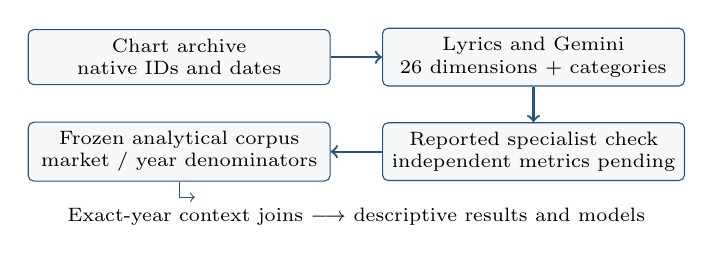
\begin{tikzpicture}[font=\scriptsize,box/.style={draw=blue,rounded corners=2pt,fill=blue!4,align=center,minimum height=7mm,text width=36mm}]
\node[box] (a) at (0,0) {Chart archive\\native IDs and dates};
\node[box] (b) at (4.5,0) {Lyrics and Gemini\\26 dimensions + categories};
\node[box] (c) at (4.5,-1.2) {Reported specialist check\\independent metrics pending};
\node[box] (d) at (0,-1.2) {Frozen analytical corpus\\market / year denominators};
\draw[->,thick,blue] (a)--(b);
\draw[->,thick,blue] (b)--(c);
\draw[->,thick,blue] (c)--(d);
\node[font=\scriptsize,align=center] at (2.25,-2.03) {Exact-year context joins $\longrightarrow$ descriptive results and models};
\draw[->,blue] (d.south)--(0,-1.78)--(.2,-1.78);
\end{tikzpicture}
\caption{Research workflow. Source records and model histories remain traceable; the analytical joins use explicit recording and time keys.}
\label{fig:workflow}
\end{figure}

The project lead reported that specialists completed a check of classifications and lyric-to-recording links. The archived confirmation does not include the number of reviewed items, individual reviewer scores or error counts. It therefore cannot establish measured classification accuracy. An earlier review contained 58 candidates and 22 AI-assisted text inspections, without an independent human reference set. Its blank review fields cannot support agreement or F1 estimates. The analytical freeze uses the latest result per document for the fixed model, taxonomy and prompt, then selects the latest applicable recording result. Text hashes, research authorization and existing exclusion decisions define the eligible version. No confidence cutoff is applied.

A separate validation package contains 3,381 provisional recordings and blind scoring sheets for two independent reviewers. No scores have yet been entered. The draw spans market, broad genre and thematic intensity, excluding the earlier 58 review documents. Language is not known for each lyric, so the draw must be revised after languages are confirmed. Reviewers qualified in those languages will independently check recording identity and score the themes, then resolve disagreements through documented adjudication. The protocol reports agreement, error patterns and performance for clearly present themes. Precision asks how often a model-positive label is correct; recall asks how many human-positive items it finds; F1 combines the two. Weighted kappa assesses ordinal agreement, while absolute error measures the size of score differences. The protocol specifies sampling weights and recording-level uncertainty intervals. These accuracy measures have not yet been estimated.

The freeze is 11 October 2026, 23:39 UTC (20:39 in S\~ao Paulo). Before geographical restrictions, the selected classification population contains 154,995 lyric documents representing 154,964 recording identities and 154,942 linked native IDs. Figure~\ref{fig:themes} uses these 154,964 identities as its pooled reference. Market analyses instead use the 153,501 recording IDs linked to the eligible geographical corpus. The two numbers describe different populations. Source-stage eligibility states and document-to-recording mappings are documented separately in the frozen manifest.

Scores run from 0 (absent) to 3 (central). A score of 2 or 3 means that a theme is clearly present. Each percentage is the share of classified recording IDs meeting this threshold. Each ID counts once per market and year. Excluded recordings remain in the selection flow and are never treated as theme absence. The scores describe the text, not the artist's conduct. Separate fields record consent and whether antisocial content is condemned, neutral, ambivalent, normalized or glorified.

\subsection{Chart dynamics and external context}
Persistence counts days in the charts, including re-entries. Calendar span is reported separately. Top-50 renewal uses Jaccard distance between adjacent daily charts: how much the two sets of recordings differ. Comparisons across missing dates are excluded. Genre tags come from artist metadata and can overlap, so their shares need not sum to 100\%.

International trends use the same 55 markets in all five complete years, with at least 300 classified recording IDs and 50\% classification coverage in every market--year. Each market has equal weight. Interquartile ranges describe market dispersion, not confidence intervals. The source sensitivities use 52 balanced Top-200 markets, 51 MGD-only markets, and 55 Viral-50 markets. The chart-family comparison uses the same 52 markets in both families. Additional panels require 70\% classification coverage throughout (8 markets), or pre-existing chart eligibility and a 1 January 2017 source start (46 markets). A distinct-recording yearly pool counts each ID once across the 55 markets. All denominators and membership lists are exported. Partial 2022 is excluded.

A further analysis links the frozen classifications to 17,268,835 daily MGD chart entries in the same 51 markets during 2017--2021. Identical duplicate entries are counted once. Source files are preserved. Each market--year is measured three ways: one vote per recording, weight by days in the charts, and weight by recorded chart streams. Each measure uses its own classified denominator and coverage. Genre profiles use the eight largest Brazilian artist-derived tags, selected by recording count before examining theme scores. Social indicators are also compared with all three weightings using the same complete-data markets within each comparison.

Context is joined by exact market and reference year: World Bank income, Gini, unemployment, population and internet indicators; UNDP Gender Inequality Index (GII); OECD SIGI for its 2019 edition. And UNODC homicide indicators~\cite{wdi,gii,sigi,homicide}. Missing values stay missing, without interpolation. SIGI is not converted into an annual time series. OONI connectivity tests are kept separately from music and search measures. The contextual export verifies unique keys, value ranges, and raw-response hashes.

Google Trends exports retain term, language, query batch, sampling period, and raw hash. The historical panel has 2,150 series--year summaries from 383 local term/language/batch series. Means are weighted by the days represented by each bucket. Weeks crossing years are split. Values reported as $<1$ contribute bounds $[0,1)$ rather than an invented point estimate. The index is relative search interest, normalized to the query's place and period, not visits or counts of people~\cite{trends}.

\subsection{Regional comparisons and repertoire composition}
We compare 2017 with 2021 in the fixed 55-market panel. Regional summaries give each market equal weight and retain a fixed membership: Latin America (16), Nordic countries (5), Japan and Taiwan (2 markets), Southeast Asia (5), six Anglophone markets and the 21 remaining panel markets. Membership lists are exported. These groups describe the available panel; they are not representative samples of entire world regions.

For each theme, a symmetric decomposition separates changes within repertoire groups from changes in the groups' shares. The within-group term weights the change in thematic prevalence by the group's average share in the two years. The composition term weights the change in group share by its average thematic prevalence. Their sum exactly reproduces the total change. We calculate this separately by broad genre and catalogue release group, within each market, then average markets. The two decompositions answer different questions and must not be added together.

Overlapping artist tags are assigned to one broad genre through a fixed priority rule published in the analysis script; untagged songs remain a group. Genre tags cover 55.8\% of the 199,496 classified endpoint recording--market--year observations. Catalogue release dates cover 75.3\%; dates later than the recording's first chart year are treated as unknown. Release groups are through 2016, 2017--2018, 2019--2020, 2021 onward and unknown. Catalogue dates can refer to editions or reissues rather than first artistic release. When a group appears in only one endpoint, its contribution is assigned to composition, with no invented within-group change. Actual lyric languages are absent, so no language decomposition is claimed.

Regional changes and decomposition terms have 95\% intervals from 400 recording-level Poisson bootstrap replicates, using seed 20261012. This procedure recalculates the results while randomly changing the weight given to each recording. One recording always receives the same weight in all its markets and years, so an international hit is not treated as many independent songs. The interval contains the middle 95\% of recalculated estimates. It describes uncertainty conditional on the observed markets and frozen AI labels. It does not include unmeasured classification error or establish population-level cultural change.

\subsection{Theme clusters and chart persistence}
We cluster the 68 markets using all 26 theme percentages from the combined historical period, 2017 through 13 March 2022. We standardize each dimension across markets before Ward hierarchical clustering, compare two through eight clusters and choose the largest mean silhouette score, a measure of separation. This is an exploratory summary without external or resampling-based cluster validation.

Longevity uses the classified MGD Top-200 panel in 51 markets. We sum observed daily chart appearances from 2017 through 2021 for each recording--market pair, counting re-entries. The dataset contains 224,598 pairs and 78,275 recording IDs. Themes can overlap. A linear model of log(1 + chart days) includes indicators for romance, explicitness and conspicuous consumption together, plus market, first observed chart year, broad genre and catalogue release-group effects. Standard errors group all appearances of a recording together across markets. Songs already charting at the start or still charting at the end have incomplete lifetimes; the outcome is observed chart presence, not a survival estimate or a causal effect of lyrical content.


\section{Results}
\subsection{Thematic profile and market differences}
Figure~\ref{fig:themes} reports all 26 dimensions. Romantic affection (35.5\%) and heartbreak (21.4\%) are the most frequent clearly present themes in the full selected corpus. Money references (16.5\%), reciprocity (14.1\%), drugs/alcohol (13.7\%), and materialism (13.5\%) follow. Sexual explicitness is 7.2\%, objectification 5.8\%, and misogyny 3.4\%. Themes overlap: their percentages do not sum to 100\%.

Brazil's all-history repertoire contains 7,186 classified IDs. Romantic affection is 40.3\%, heartbreak 24.1\%, casual sex 15.1\%, explicitness 12.5\%, objectification 7.1\%, misogyny 1.9\%, and materialism 8.6\%. Brazil therefore combines comparatively frequent sexual and romantic content with lower misogyny and materialism than several comparator repertoires (Table~\ref{tab:markets}). Sexual content and misogyny do not move as one measure.

\begin{figure}[t]
\centering
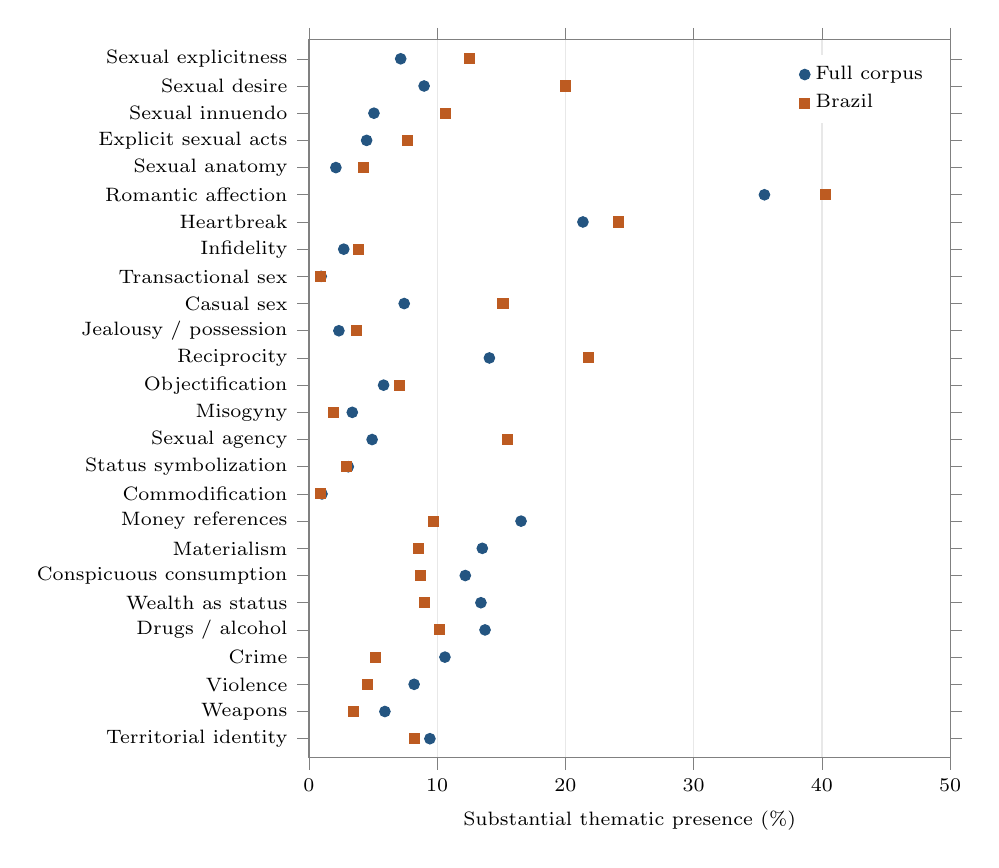
\begin{tikzpicture}
\begin{axis}[width=\dimexpr\columnwidth-24mm\relax,height=107mm,scale only axis=false,
 xmin=0,xmax=50,ymin=.3,ymax=26.7,
 xlabel={Substantial thematic presence (\%)},
 xlabel style={font=\scriptsize},xtick={0,10,20,30,40,50},
 ytick={26,25,24,23,22,21,20,19,18,17,16,15,14,13,12,11,10,9,8,7,6,5,4,3,2,1},yticklabels={{Sexual explicitness},{Sexual desire},{Sexual innuendo},{Explicit sexual acts},{Sexual anatomy},{Romantic affection},{Heartbreak},{Infidelity},{Transactional sex},{Casual sex},{Jealousy / possession},{Reciprocity},{Objectification},{Misogyny},{Sexual agency},{Status symbolization},{Commodification},{Money references},{Materialism},{Conspicuous consumption},{Wealth as status},{Drugs / alcohol},{Crime},{Violence},{Weapons},{Territorial identity}},
 tick label style={font=\scriptsize},axis line style={gray},
 xmajorgrids=true,grid style={gray!18},tick align=outside,
 legend style={at={(.98,.98)},anchor=north east,font=\scriptsize,draw=none,fill=white},
 legend cell align=left]
\addplot[only marks,mark=*,mark size=1.9pt,color=blue] coordinates {(7.15134,26) (8.97628,25) (5.06505,24) (4.49395,23) (2.09791,22) (35.51341,21) (21.35980,20) (2.71160,19) (0.95248,18) (7.42430,17) (2.33215,16) (14.06649,15) (5.81748,14) (3.37562,13) (4.92179,12) (3.06394,11) (1.01378,10) (16.53481,9) (13.51475,8) (12.18864,7) (13.40634,6) (13.72706,5) (10.60053,4) (8.19803,3) (5.91944,2) (9.42800,1)};
\addlegendentry{Full corpus}
\addplot[only marks,mark=square*,mark size=1.8pt,color=orange] coordinates {(12.51044,26) (20.01113,25) (10.65962,24) (7.65377,23) (4.28611,22) (40.28667,21) (24.13025,20) (3.86863,19) (0.91845,18) (15.12664,17) (3.67381,16) (21.80629,15) (7.08322,14) (1.89257,13) (15.47453,12) (2.90843,11) (0.93237,10) (9.68550,9) (8.55831,8) (8.72530,7) (9.01753,6) (10.17256,5) (5.17673,4) (4.53660,3) (3.46507,2) (8.21041,1)};
\addlegendentry{Brazil}
\end{axis}
\end{tikzpicture}
\caption{How Brazil's lyrical profile compares with the pooled reference. Each point shows the percentage of recordings in which a theme is clearly present. Blue circles count 154,964 selected identities once, before geographical restrictions; orange squares count Brazil's 7,186 classified IDs once. Market analyses elsewhere use 153,501 IDs after geographical restrictions. The pooled reference is not an average of country percentages, and overlapping themes need not sum to 100\%.}
\label{fig:themes}
\end{figure}

\begin{table}[t]
\caption{Selected circulation markets, combined historical period. $n$: classified recording IDs; E: explicitness; C: casual sex; M: misogyny; Mat.: materialism. All thematic columns are percentages at intensity $\geq2$.}
\label{tab:markets}
\centering\footnotesize\setlength{\tabcolsep}{3.5pt}
\begin{tabular}{@{}lrrrrr@{}}
\toprule Market & $n$ & E & C & M & Mat.\\
\midrule
BR & 7,186 & 12.5 & 15.1 & 1.9 & 8.6 \\
US & 11,296 & 16.1 & 15.2 & 8.3 & 24.5 \\
GB & 10,752 & 10.9 & 10.9 & 3.8 & 17.9 \\
DE & 11,907 & 9.4 & 8.9 & 7.2 & 27.7 \\
FR & 11,579 & 10.3 & 8.7 & 6.8 & 23.0 \\
ES & 8,082 & 11.4 & 13.6 & 1.6 & 10.3 \\
PT & 8,065 & 11.9 & 12.6 & 3.8 & 14.2 \\
JP & 8,047 & 3.6 & 3.7 & 0.8 & 4.9 \\
\bottomrule
\end{tabular}
\end{table}

Across all 68 markets, the largest explicitness shares are in the Dominican Republic (21.4\%), Panama (19.2\%), and Chile (17.6\%). The largest misogyny share is in Romania (11.1\%). The largest materialism share is in Switzerland (27.8\%). These are distributions of charted recordings under a common coding rule, not rankings of national character.

Themes are distinct but overlap. Of 11,082 recordings with substantial explicitness, 60.1\% also have substantial objectification and 30.8\% misogyny. Among 20,943 materialism-positive recordings, 40.7\% also code crime. Among 12,704 violence-positive recordings, 78.3\% also code crime. These conditional shares concern texts, not people. Consent, representation and stance remain separate measures in the accompanying distributions.

\subsection{Brazil over time and repertoire persistence}
From 2017 to 2021, Brazil's explicitness share rises from 7.0\% to 19.7\% and casual-sex share from 8.2\% to 23.8\%. Romantic affection stays near 40--42\% (Figure~\ref{fig:brazil}). These are changes in each year's repertoire. Repeated recordings may enter several annual denominators. The 2022 partial window is shown separately and is not a full-year continuation.

\begin{figure}[t]
\centering
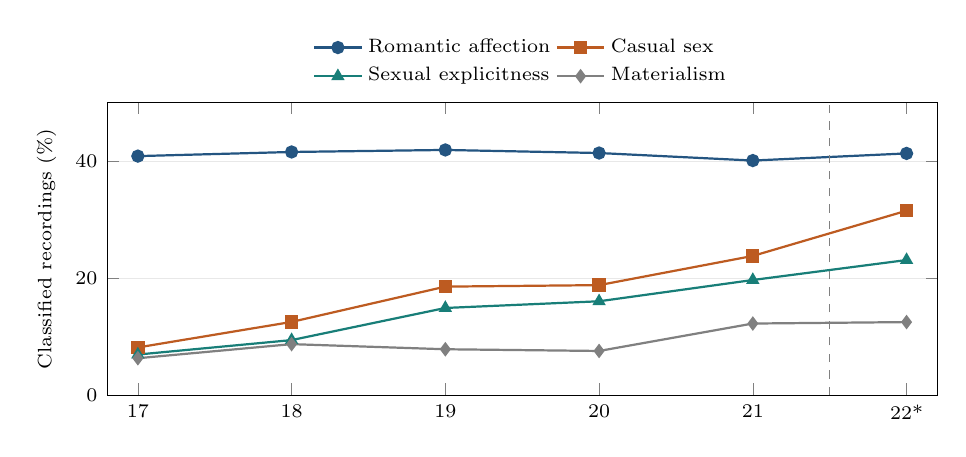
\begin{tikzpicture}
\begin{axis}[width=\columnwidth,height=53mm,xmin=2016.8,xmax=2022.2,ymin=0,ymax=50,
 xtick={2017,2018,2019,2020,2021,2022},xticklabels={17,18,19,20,21,22*},
 ylabel={Classified recordings (\%)},ylabel style={font=\scriptsize},
 tick label style={font=\scriptsize},ymajorgrids=true,grid style={gray!18},
 legend style={at={(.5,1.02)},anchor=south,legend columns=2,font=\scriptsize,draw=none},
 legend cell align=left]
\addplot[color=blue,mark=*,thick] coordinates {(2017,40.84381) (2018,41.55172) (2019,41.89627) (2020,41.37199) (2021,40.08499) (2022,41.30435)};\addlegendentry{Romantic affection}
\addplot[color=orange,mark=square*,thick] coordinates {(2017,8.16876) (2018,12.52874) (2019,18.55754) (2020,18.81188) (2021,23.79603) (2022,31.52174)};\addlegendentry{Casual sex}
\addplot[color=teal,mark=triangle*,thick] coordinates {(2017,6.95691) (2018,9.42529) (2019,14.91086) (2020,16.05375) (2021,19.68839) (2022,23.09783)};\addlegendentry{Sexual explicitness}
\addplot[color=gray,mark=diamond*,thick] coordinates {(2017,6.32855) (2018,8.73563) (2019,7.86062) (2020,7.56719) (2021,12.25212) (2022,12.50000)};\addlegendentry{Materialism}
\draw[gray,dashed] (axis cs:2021.5,0)--(axis cs:2021.5,50);
\end{axis}
\end{tikzpicture}
\caption{Brazil's annual thematic shares. Classified denominators for 2017--2022: 2,228; 1,740; 1,234; 1,414; 1,412; 368. *2022 ends on 13 March. Lines connect annual summaries, not individual song trajectories.}
\label{fig:brazil}
\end{figure}

In the separate MGD Top-200 dynamics dataset, Brazil has 5,010 distinct recording--market pairs, with a median of 16 chart days (interquartile range 2--98), compared with 6 in the United States and United Kingdom, 7 in Germany, and 13 in Japan. Brazil's mean Top-50 Jaccard turnover is 0.069 across 1,892 adjacent daily chart pairs, against 0.114 in the United States and 0.032 in Japan. This supports a description of different repertoire persistence, without treating turnover as psychological anxiety.

Genre profiles are examined alongside exposure below. Artist rankings and network files remain supplementary descriptions rather than additional independent song samples.

\subsection{International shifts and new patterns}
\begin{figure*}[t]
\centering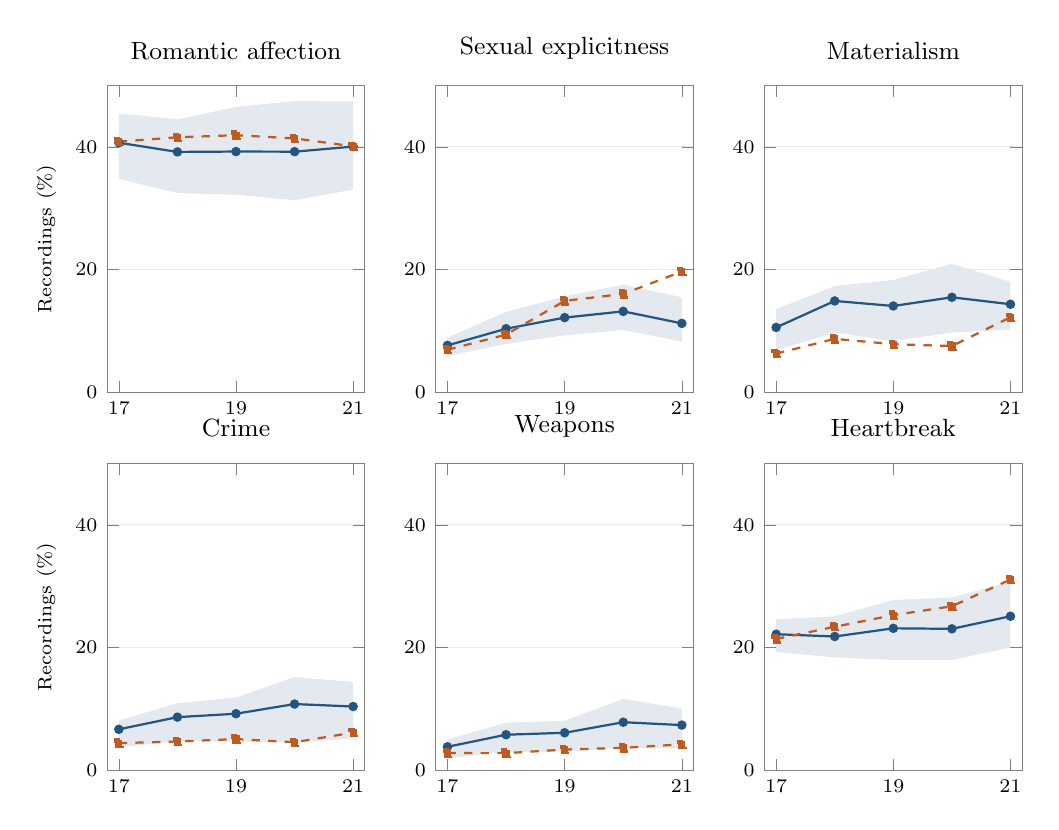
\begin{tikzpicture}
\begin{groupplot}[group style={group size=3 by 2,horizontal sep=9mm,vertical sep=9mm},
 width=.27\textwidth,height=39mm,scale only axis=true,
 xmin=2016.8,xmax=2021.2,ymin=0,ymax=50,xtick={2017,2019,2021},xticklabels={17,19,21},ytick={0,20,40},
 tick label style={font=\scriptsize},title style={font=\small},ylabel style={font=\scriptsize},
 axis line style={gray},ymajorgrids=true,grid style={gray!18}]
\nextgroupplot[title={Romantic affection},ylabel={Recordings (\%)}]
\addplot[name path=lower0,draw=none] coordinates {(2017.000000,34.771657) (2018.000000,32.469527) (2019.000000,32.204276) (2020.000000,31.313403) (2021.000000,33.037893)};
\addplot[name path=upper0,draw=none] coordinates {(2017.000000,45.437784) (2018.000000,44.472891) (2019.000000,46.480589) (2020.000000,47.452949) (2021.000000,47.384528)};
\addplot[blue!13,draw=none] fill between[of=lower0 and upper0];
\addplot[blue,thick,mark=*,mark size=1.3pt] coordinates {(2017.000000,40.667626) (2018.000000,39.169534) (2019.000000,39.231390) (2020.000000,39.211221) (2021.000000,40.038148)};
\addplot[orange,thick,dashed,mark=square*,mark size=1.3pt] coordinates {(2017.000000,40.843806) (2018.000000,41.551724) (2019.000000,41.896272) (2020.000000,41.371994) (2021.000000,40.084986)};
\nextgroupplot[title={Sexual explicitness},ylabel={}]
\addplot[name path=lower1,draw=none] coordinates {(2017.000000,5.909948) (2018.000000,7.916010) (2019.000000,9.312452) (2020.000000,10.167596) (2021.000000,8.295344)};
\addplot[name path=upper1,draw=none] coordinates {(2017.000000,8.914187) (2018.000000,13.132479) (2019.000000,15.643946) (2020.000000,17.565024) (2021.000000,15.501254)};
\addplot[blue!13,draw=none] fill between[of=lower1 and upper1];
\addplot[blue,thick,mark=*,mark size=1.3pt] coordinates {(2017.000000,7.667900) (2018.000000,10.380642) (2019.000000,12.192882) (2020.000000,13.209204) (2021.000000,11.254716)};
\addplot[orange,thick,dashed,mark=square*,mark size=1.3pt] coordinates {(2017.000000,6.956912) (2018.000000,9.425287) (2019.000000,14.910859) (2020.000000,16.053748) (2021.000000,19.688385)};
\nextgroupplot[title={Materialism},ylabel={}]
\addplot[name path=lower2,draw=none] coordinates {(2017.000000,6.863643) (2018.000000,9.763686) (2019.000000,8.354031) (2020.000000,9.764218) (2021.000000,10.235561)};
\addplot[name path=upper2,draw=none] coordinates {(2017.000000,13.590013) (2018.000000,17.333145) (2019.000000,18.312764) (2020.000000,20.959022) (2021.000000,17.996222)};
\addplot[blue!13,draw=none] fill between[of=lower2 and upper2];
\addplot[blue,thick,mark=*,mark size=1.3pt] coordinates {(2017.000000,10.590463) (2018.000000,14.908394) (2019.000000,14.086727) (2020.000000,15.500047) (2021.000000,14.370067)};
\addplot[orange,thick,dashed,mark=square*,mark size=1.3pt] coordinates {(2017.000000,6.328546) (2018.000000,8.735632) (2019.000000,7.860616) (2020.000000,7.567185) (2021.000000,12.252125)};
\nextgroupplot[title={Crime},ylabel={Recordings (\%)}]
\addplot[name path=lower3,draw=none] coordinates {(2017.000000,3.751466) (2018.000000,4.795346) (2019.000000,4.711368) (2020.000000,4.533178) (2021.000000,5.213941)};
\addplot[name path=upper3,draw=none] coordinates {(2017.000000,8.122014) (2018.000000,10.944824) (2019.000000,11.878786) (2020.000000,15.202549) (2021.000000,14.404351)};
\addplot[blue!13,draw=none] fill between[of=lower3 and upper3];
\addplot[blue,thick,mark=*,mark size=1.3pt] coordinates {(2017.000000,6.696014) (2018.000000,8.678108) (2019.000000,9.234035) (2020.000000,10.810769) (2021.000000,10.406582)};
\addplot[orange,thick,dashed,mark=square*,mark size=1.3pt] coordinates {(2017.000000,4.443447) (2018.000000,4.712644) (2019.000000,5.105348) (2020.000000,4.596888) (2021.000000,6.161473)};
\nextgroupplot[title={Weapons},ylabel={}]
\addplot[name path=lower4,draw=none] coordinates {(2017.000000,1.989334) (2018.000000,3.036415) (2019.000000,3.045682) (2020.000000,3.684788) (2021.000000,3.565187)};
\addplot[name path=upper4,draw=none] coordinates {(2017.000000,5.030013) (2018.000000,7.771171) (2019.000000,8.074075) (2020.000000,11.641704) (2021.000000,10.062843)};
\addplot[blue!13,draw=none] fill between[of=lower4 and upper4];
\addplot[blue,thick,mark=*,mark size=1.3pt] coordinates {(2017.000000,3.849540) (2018.000000,5.817621) (2019.000000,6.129526) (2020.000000,7.851988) (2021.000000,7.383677)};
\addplot[orange,thick,dashed,mark=square*,mark size=1.3pt] coordinates {(2017.000000,2.827648) (2018.000000,2.816092) (2019.000000,3.403566) (2020.000000,3.677511) (2021.000000,4.249292)};
\nextgroupplot[title={Heartbreak},ylabel={}]
\addplot[name path=lower5,draw=none] coordinates {(2017.000000,19.287839) (2018.000000,18.413000) (2019.000000,17.997344) (2020.000000,17.984207) (2021.000000,20.012556)};
\addplot[name path=upper5,draw=none] coordinates {(2017.000000,24.584372) (2018.000000,25.113938) (2019.000000,27.742375) (2020.000000,28.169940) (2021.000000,30.729568)};
\addplot[blue!13,draw=none] fill between[of=lower5 and upper5];
\addplot[blue,thick,mark=*,mark size=1.3pt] coordinates {(2017.000000,22.184707) (2018.000000,21.807672) (2019.000000,23.141389) (2020.000000,23.056031) (2021.000000,25.105022)};
\addplot[orange,thick,dashed,mark=square*,mark size=1.3pt] coordinates {(2017.000000,21.409336) (2018.000000,23.390805) (2019.000000,25.283630) (2020.000000,26.732673) (2021.000000,31.090652)};
\end{groupplot}\end{tikzpicture}
\caption{International trajectories, 2017--2021. Blue circles: equal-market means for the same 55 markets in all five years; orange dashed squares: Brazil. Bands are the middle 50\% of market values, not confidence intervals. Each theme uses the same 0--50\% axis; substantial presence means intensity $\geq2$. Markets have at least 300 classified recordings and 50\% classification coverage in every year. The changing annual repertoires, not changes within a song, are measured.}
\label{fig:global-time}
\end{figure*}
\begin{figure*}[t]
\centering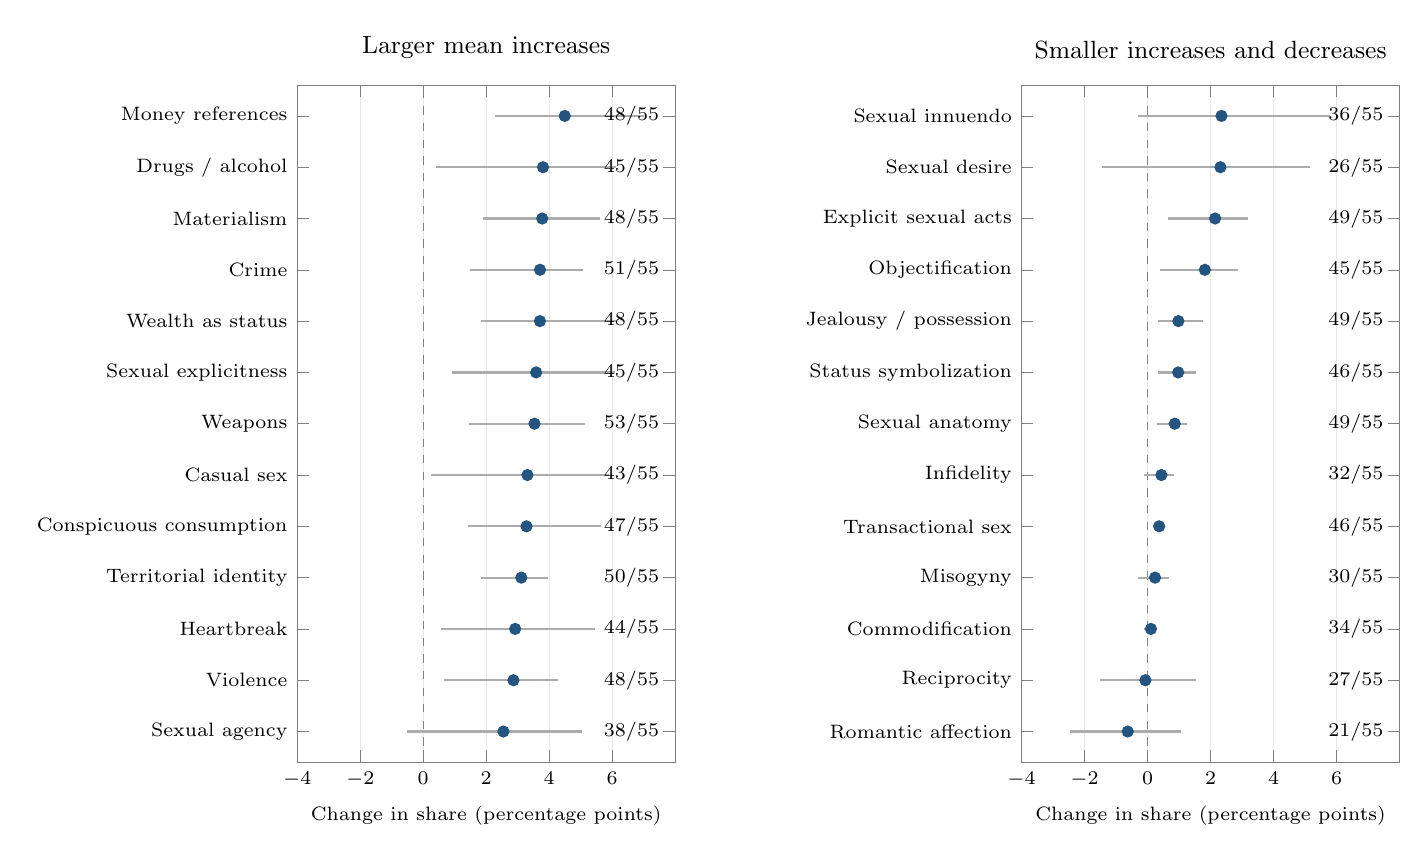
\begin{tikzpicture}
\begin{groupplot}[group style={group size=2 by 1,horizontal sep=44mm},
width=48mm,height=86mm,scale only axis=true,xmin=-4,xmax=8,ymin=.4,ymax=13.6,
xtick={-4,-2,0,2,4,6},xlabel={Change in share (percentage points)},
xlabel style={font=\scriptsize},tick label style={font=\scriptsize},title style={font=\small},
xmajorgrids=true,grid style={gray!18},axis line style={gray}]
\nextgroupplot[ytick={13,12,11,10,9,8,7,6,5,4,3,2,1},yticklabels={{Money references},{Drugs / alcohol},{Materialism},{Crime},{Wealth as status},{Sexual explicitness},{Weapons},{Casual sex},{Conspicuous consumption},{Territorial identity},{Heartbreak},{Violence},{Sexual agency}},title={Larger mean increases}]
\draw[gray,dashed] (axis cs:0,.4)--(axis cs:0,13.6);
\draw[gray!65,thick] (axis cs:2.267652,13)--(axis cs:7.022541,13);
\node[font=\scriptsize,anchor=east] at (axis cs:7.8,13) {48/55};
\draw[gray!65,thick] (axis cs:0.410851,12)--(axis cs:6.117446,12);
\node[font=\scriptsize,anchor=east] at (axis cs:7.8,12) {45/55};
\draw[gray!65,thick] (axis cs:1.901706,11)--(axis cs:5.611154,11);
\node[font=\scriptsize,anchor=east] at (axis cs:7.8,11) {48/55};
\draw[gray!65,thick] (axis cs:1.477499,10)--(axis cs:5.067675,10);
\node[font=\scriptsize,anchor=east] at (axis cs:7.8,10) {51/55};
\draw[gray!65,thick] (axis cs:1.839363,9)--(axis cs:6.126683,9);
\node[font=\scriptsize,anchor=east] at (axis cs:7.8,9) {48/55};
\draw[gray!65,thick] (axis cs:0.900828,8)--(axis cs:6.093631,8);
\node[font=\scriptsize,anchor=east] at (axis cs:7.8,8) {45/55};
\draw[gray!65,thick] (axis cs:1.440705,7)--(axis cs:5.143227,7);
\node[font=\scriptsize,anchor=east] at (axis cs:7.8,7) {53/55};
\draw[gray!65,thick] (axis cs:0.252737,6)--(axis cs:5.901170,6);
\node[font=\scriptsize,anchor=east] at (axis cs:7.8,6) {43/55};
\draw[gray!65,thick] (axis cs:1.428501,5)--(axis cs:5.661177,5);
\node[font=\scriptsize,anchor=east] at (axis cs:7.8,5) {47/55};
\draw[gray!65,thick] (axis cs:1.837014,4)--(axis cs:3.978834,4);
\node[font=\scriptsize,anchor=east] at (axis cs:7.8,4) {50/55};
\draw[gray!65,thick] (axis cs:0.574003,3)--(axis cs:5.449409,3);
\node[font=\scriptsize,anchor=east] at (axis cs:7.8,3) {44/55};
\draw[gray!65,thick] (axis cs:0.670765,2)--(axis cs:4.292003,2);
\node[font=\scriptsize,anchor=east] at (axis cs:7.8,2) {48/55};
\draw[gray!65,thick] (axis cs:-0.518891,1)--(axis cs:5.030915,1);
\node[font=\scriptsize,anchor=east] at (axis cs:7.8,1) {38/55};
\addplot[only marks,blue,mark=*,mark size=2pt] coordinates {(4.495539,13) (3.804479,12) (3.779604,11) (3.710568,10) (3.707348,9) (3.586817,8) (3.534137,7) (3.309420,6) (3.279988,5) (3.115725,4) (2.920314,3) (2.865182,2) (2.548219,1)};
\nextgroupplot[ytick={13,12,11,10,9,8,7,6,5,4,3,2,1},yticklabels={{Sexual innuendo},{Sexual desire},{Explicit sexual acts},{Objectification},{Jealousy / possession},{Status symbolization},{Sexual anatomy},{Infidelity},{Transactional sex},{Misogyny},{Commodification},{Reciprocity},{Romantic affection}},title={Smaller increases and decreases}]
\draw[gray,dashed] (axis cs:0,.4)--(axis cs:0,13.6);
\draw[gray!65,thick] (axis cs:-0.318277,13)--(axis cs:5.790287,13);
\node[font=\scriptsize,anchor=east] at (axis cs:7.8,13) {36/55};
\draw[gray!65,thick] (axis cs:-1.446731,12)--(axis cs:5.155236,12);
\node[font=\scriptsize,anchor=east] at (axis cs:7.8,12) {26/55};
\draw[gray!65,thick] (axis cs:0.638187,11)--(axis cs:3.174208,11);
\node[font=\scriptsize,anchor=east] at (axis cs:7.8,11) {49/55};
\draw[gray!65,thick] (axis cs:0.385005,10)--(axis cs:2.858504,10);
\node[font=\scriptsize,anchor=east] at (axis cs:7.8,10) {45/55};
\draw[gray!65,thick] (axis cs:0.321588,9)--(axis cs:1.761613,9);
\node[font=\scriptsize,anchor=east] at (axis cs:7.8,9) {49/55};
\draw[gray!65,thick] (axis cs:0.319422,8)--(axis cs:1.538841,8);
\node[font=\scriptsize,anchor=east] at (axis cs:7.8,8) {46/55};
\draw[gray!65,thick] (axis cs:0.296223,7)--(axis cs:1.264193,7);
\node[font=\scriptsize,anchor=east] at (axis cs:7.8,7) {49/55};
\draw[gray!65,thick] (axis cs:-0.129502,6)--(axis cs:0.841650,6);
\node[font=\scriptsize,anchor=east] at (axis cs:7.8,6) {32/55};
\draw[gray!65,thick] (axis cs:0.182799,5)--(axis cs:0.485998,5);
\node[font=\scriptsize,anchor=east] at (axis cs:7.8,5) {46/55};
\draw[gray!65,thick] (axis cs:-0.294200,4)--(axis cs:0.667159,4);
\node[font=\scriptsize,anchor=east] at (axis cs:7.8,4) {30/55};
\draw[gray!65,thick] (axis cs:-0.112472,3)--(axis cs:0.256888,3);
\node[font=\scriptsize,anchor=east] at (axis cs:7.8,3) {34/55};
\draw[gray!65,thick] (axis cs:-1.495781,2)--(axis cs:1.526836,2);
\node[font=\scriptsize,anchor=east] at (axis cs:7.8,2) {27/55};
\draw[gray!65,thick] (axis cs:-2.478436,1)--(axis cs:1.060692,1);
\node[font=\scriptsize,anchor=east] at (axis cs:7.8,1) {21/55};
\addplot[only marks,blue,mark=*,mark size=2pt] coordinates {(2.345754,13) (2.312660,12) (2.142570,11) (1.817757,10) (0.977507,9) (0.972531,8) (0.863537,7) (0.437759,6) (0.367759,5) (0.235336,4) (0.106954,3) (-0.070506,2) (-0.629478,1)};
\end{groupplot}\end{tikzpicture}
\caption{Which themes increased, and how widely? All 26 dimensions are ordered by mean change from 2017 to 2021 and split across two panels with the same scale. A blue point to the right of zero indicates an increase in the average market share. Gray bars show the middle half of market changes, not confidence intervals. Counts at the right show how many of the same 55 markets increased. Materialism, crime and weapons rose in most markets, whereas a positive mean for sexual desire masks a less widespread change.}
\label{fig:global-changes}
\end{figure*}
\begin{figure}[t]
\centering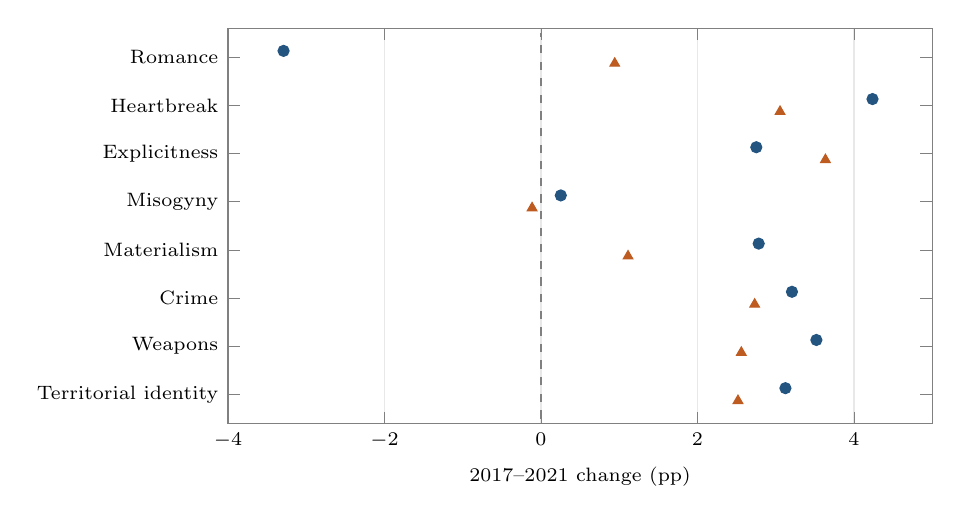
\begin{tikzpicture}
\begin{axis}[width=\dimexpr\columnwidth-16mm\relax,height=66mm,
 xmin=-4,xmax=5,ymin=.4,ymax=8.6,xtick={-4,-2,0,2,4},ytick={8,7,6,5,4,3,2,1},
 yticklabels={Romance,Heartbreak,Explicitness,Misogyny,Materialism,Crime,Weapons,Territorial identity},
 xlabel={2017--2021 change (pp)},xlabel style={font=\scriptsize},tick label style={font=\scriptsize},
 xmajorgrids=true,grid style={gray!18},axis line style={gray}]
\draw[gray,dashed] (axis cs:0,.5)--(axis cs:0,8.5);
\addplot[only marks,blue,mark=*,mark size=2pt] coordinates {(-3.289687,8.130) (4.237042,7.130) (2.752028,6.130) (0.253379,5.130) (2.782451,4.130) (3.207601,3.130) (3.519905,2.130) (3.124103,1.130)};
\addplot[only marks,orange,mark=triangle*,mark size=2pt] coordinates {(0.942803,7.870) (3.055312,6.870) (3.635211,5.870) (-0.113495,4.870) (1.112607,3.870) (2.731079,2.870) (2.560362,1.870) (2.517819,0.870)};
\end{axis}\end{tikzpicture}
\caption{Chart-family contrast in the same 52 markets. Blue circles: Top 200 (source union, IDs deduplicated); orange triangles: Viral 50. Each panel has at least 300 classified IDs and 50\% classification coverage in every full year. The romance trend changes direction across chart families; growth of status and conflict themes persists.}
\label{fig:family-trends}
\end{figure}

Status and conflict gain repertoire share. In the fixed 55-market panel, mean substantial money references increase by 4.50 percentage points (pp), drugs/alcohol by 3.80, materialism by 3.78, crime by 3.71, weapons by 3.53 and territorial identity by 3.12 from 2017 to 2021 (Figures~\ref{fig:global-time}--\ref{fig:global-changes}). Growth is geographically broad: weapons increase in 53/55 markets, crime in 51/55, territorial identity in 50/55, and materialism in 48/55. This is a shift in chart repertoire composition, not a claim that listeners changed their conduct.

Romance persists while heartbreak grows. Romantic affection averages 40.67\% in 2017 and 40.04\% in 2021. Heartbreak rises from 22.18\% to 25.11\% in 44 markets. Sexual explicitness rises from 7.67\% to 11.25\%, whereas misogyny changes only from 2.71\% to 2.95\%. These trajectories separate affection, suffering, sexual content and gender hostility rather than treating them as one process.

Mean growth can be geographically concentrated. Sexual desire has a positive mean change (+2.31 pp), yet its median market change is $-0.09$ pp and only 26/55 markets increase. Large shifts in a subset of markets raise the mean. Figure~\ref{fig:global-changes} separates average magnitude from geographical breadth.

Brazil's strongest shifts differ from the international pattern. Brazil has the largest casual-sex increase in the 55-market panel (+15.63 pp), the second-largest explicitness increase (+12.73 pp, after Andorra), and the third-largest heartbreak increase (+9.68 pp, after Paraguay and Bolivia). Its weapons increase (+1.42 pp) is smaller than the international mean (+3.53 pp). Brazil's change therefore concentrates on sexual and relational themes rather than reproducing the strongest conflict trend.

The aggregate masks chart-family divergence. For the same 52 markets, romance falls by 3.29 pp in Top 200 but rises by 0.94 pp in Viral 50 (Figure~\ref{fig:family-trends}). Heartbreak grows in both (+4.24 and +3.06 pp), as do materialism (+2.78 and +1.11) and weapons (+3.52 and +2.56). Near-flat aggregate romance is therefore not evidence of an unchanged chart landscape. Misogyny also differs slightly in direction (+0.25 versus $-0.11$ pp).

Growth of materialism, crime, weapons, heartbreak and territorial identity persists in every source/coverage sensitivity. The distinct-recording pool also increases in these themes: materialism rises from 8.34\% to 15.88\%, crime from 7.03\% to 13.21\%, and weapons from 3.77\% to 7.71\%. Pool and market-mean levels answer different questions. Shared recordings are not summed as independent global songs. Source-specific declines in romance remain explicit rather than being hidden by a single pooled statistic.

\subsection{What receives chart exposure, and where themes concentrate}
\begin{figure*}[t]
\centering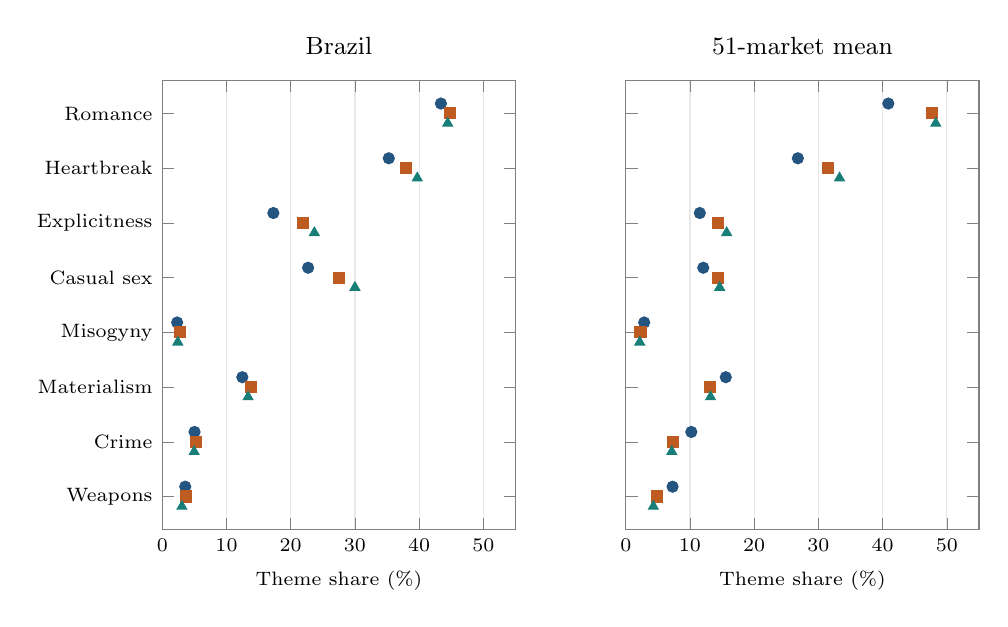
\begin{tikzpicture}
\begin{groupplot}[group style={group size=2 by 1,horizontal sep=14mm},width=.37\textwidth,height=57mm,scale only axis=true,
 xmin=0,xmax=55,ymin=.4,ymax=8.6,xtick={0,10,20,30,40,50},ytick={8,7,6,5,4,3,2,1},
 tick label style={font=\scriptsize},title style={font=\small},xlabel={Theme share (\%)},xlabel style={font=\scriptsize},
 xmajorgrids=true,grid style={gray!18},axis line style={gray}]
\nextgroupplot[title={Brazil},yticklabels={Romance,Heartbreak,Explicitness,Casual sex,Misogyny,Materialism,Crime,Weapons}]
\addplot[only marks,blue,mark=*,mark size=2pt] coordinates {(43.381643,8.18) (35.265700,7.18) (17.294686,6.18) (22.705314,5.18) (2.318841,4.18) (12.463768,3.18) (5.024155,2.18) (3.574879,1.18)};
\addplot[only marks,orange,mark=square*,mark size=2pt] coordinates {(44.788609,8.00) (37.979871,7.00) (21.901567,6.00) (27.538028,5.00) (2.718158,4.00) (13.756624,3.00) (5.192330,2.00) (3.741756,1.00)};
\addplot[only marks,teal,mark=triangle*,mark size=2pt] coordinates {(44.440178,7.82) (39.700251,6.82) (23.678509,5.82) (29.993152,4.82) (2.419407,3.82) (13.363212,2.82) (4.962364,1.82) (3.052341,0.82)};
\nextgroupplot[title={51-market mean},yticklabels={}]
\addplot[only marks,blue,mark=*,mark size=2pt] coordinates {(40.878956,8.18) (26.792659,7.18) (11.530168,6.18) (12.068266,5.18) (2.869502,4.18) (15.572504,3.18) (10.206607,2.18) (7.290892,1.18)};
\addplot[only marks,orange,mark=square*,mark size=2pt] coordinates {(47.715061,8.00) (31.445475,7.00) (14.387629,6.00) (14.313864,5.00) (2.306561,4.00) (13.119027,3.00) (7.407665,2.00) (4.890054,1.00)};
\addplot[only marks,teal,mark=triangle*,mark size=2pt] coordinates {(48.268171,7.82) (33.284715,6.82) (15.707437,5.82) (14.619290,4.82) (2.178785,3.82) (13.201071,2.82) (7.165506,1.82) (4.296835,0.82)};
\end{groupplot}\end{tikzpicture}
\caption{Three views of the same classified Top-200 repertoire in 2021. Blue circles count recording IDs equally; orange squares weight their observed chart days; teal triangles weight observed chart streams. The right panel averages the same 51 markets equally. Every denominator contains classified records only. Brazil has 1,035 recording IDs in this intended classified repertoire. The analysis describes their chart appearances and eligible streams. Sampling and exposure-denominator details are provided in the supplementary files. Streams are chart-eligible plays during chart appearances, not people or all Spotify plays.}
\label{fig:chart-exposure}
\end{figure*}
\begin{table}[t]
\caption{Brazilian genre-tag profiles, MGD Top 200, 2017--2021. The eight largest artist-derived tags are selected by charted recording count. $n$: classified IDs; R: romance; E: explicitness; C: casual sex; M: misogyny; Mat.: materialism. Theme values are percentages of classified IDs, not genre-wide population estimates. Tags overlap.}
\label{tab:genre-profiles}
\centering\scriptsize\setlength{\tabcolsep}{2.8pt}
\begin{tabular}{@{}lrrrrrr@{}}\toprule Tag & $n$ & R & E & C & M & Mat.\\\midrule
Pop & 757 & 51.7 & 5.3 & 7.8 & 0.3 & 4.1 \\
Agronejo & 283 & 61.1 & 1.1 & 9.2 & 0.0 & 0.7 \\
Arrocha & 227 & 55.9 & 7.0 & 13.7 & 0.4 & 0.9 \\
Rap / hip-hop & 106 & 16.0 & 25.5 & 21.7 & 3.8 & 40.6 \\
Brazilian funk & 141 & 25.5 & 22.0 & 29.1 & 0.7 & 5.7 \\
Sertanejo & 84 & 70.2 & 0.0 & 8.3 & 0.0 & 1.2 \\
Rock & 71 & 31.0 & 0.0 & 0.0 & 0.0 & 0.0 \\
K-pop & 55 & 34.5 & 0.0 & 0.0 & 0.0 & 9.1 \\
\bottomrule\end{tabular}
\end{table}

Counting recordings and counting plays give different pictures. In 2021, romance covers 40.9\% of classified recording IDs in the 51-market MGD panel but 48.3\% of classified chart streams. Heartbreak rises from 26.8\% to 33.3\%, and explicitness from 11.5\% to 15.7\%. Crime falls from 10.2\% to 7.2\%, weapons from 7.3\% to 4.3\%, and materialism from 15.6\% to 13.2\% when streams supply the weights (Figure~\ref{fig:chart-exposure}). Growth in the number of conflict-themed recordings therefore coexists with a smaller share of recorded plays than a song-count measure suggests. Romance remains central to both views.

Brazil's sexual and relational themes receive extra chart weight. Among its classified Top-200 repertoire in 2021, casual sex covers 22.7\% of recording IDs and 30.0\% of chart streams. Explicitness covers 17.3\% and 23.7\%. Heartbreak covers 35.3\% and 39.7\%. Misogyny stays close to 2.3--2.4\%. These are shares of classified records and their observed chart plays. The denominator includes only streams attached to the intended classified repertoire.

Genres reveal different combinations, not one national profile. Across 2017--2021, the eight largest Brazilian tag groups have distinct profiles. Sertanejo has 70.2\% romantic affection and no substantial explicitness among 84 classified IDs. Brazilian funk has 29.1\% casual sex and 22.0\% explicitness among 141 IDs, while misogyny is 0.7\%. Rap/hip-hop has 40.6\% materialism and 25.5\% explicitness among 106 IDs. Agronejo has 61.1\% romance and 1.1\% explicitness among 283. Table~\ref{tab:genre-profiles} reports every group and its coverage. Country totals combine styles with different profiles. Separating these observed groups makes the comparison more informative. The tags describe artists' genre metadata and can overlap.

Changing the weights also changes the apparent relationship with social context. A theme can occur in many different songs while accounting for a smaller share of chart plays. This makes repertoire selection a possible explanation for the original social correlations. The following analysis examines that possibility with a small set of adjusted comparisons.

\subsection{Three focused questions about social context}
Gini measures income inequality, with larger values indicating a more unequal distribution. The Gender Inequality Index (GII) measures gender disadvantage in health, empowerment and employment. PPP income adjusts purchasing power for differences in the cost of living. Homicide is measured as deaths per 100,000 people. None of these indicators directly measures what people believe about a song.
Songs can describe, criticize or imagine social conditions. Their chart presence also depends on which genres and international hits circulate. Research on cross-country listening links musical preferences to language, culture and social networks~\cite{liu}. Work on lyrical change shows why the supply and composition of songs matter~\cite{varnum,parada}. These findings motivate a selection-based interpretation: a country indicator and a lyric theme can be associated because markets contain different repertoires, even when the lyrics do not mirror residents' lives.

We therefore narrow the contextual analysis to three questions. First, does the relationship between materialism and income inequality remain after accounting for economic resources and repertoire composition? Wealth references may express aspiration or status display, but they can also be concentrated in commercially successful genres. Second, does the relationship between misogyny and the Gender Inequality Index (GII) survive adjustment for the same differences? Depicting a gender stereotype and endorsing it are separate processes, so national gender conditions need not produce more hostile lyrics. Third, does the relationship between lyrical violence and homicide persist after adjustment? Violence can be narrated, condemned or dramatized, while a market can import songs from places with very different conditions. These are competing explanations to examine, rather than reasons to predict a particular sign.

The three corresponding hypotheses concern an association that remains after accounting for measured selection: H1 pairs materialism with inequality, H2 pairs misogyny with gender conditions, and H3 pairs lyrical violence with homicide. A direct social-reflection account would predict a remaining contextual association. A repertoire-selection account would predict attenuation once economic resources, genre and shared circulation are considered. The sign is left open because depiction, criticism and aspiration can operate in different directions. These hypotheses were formulated after inspecting the original descriptive results. The analysis is exploratory and has not been preregistered. The complete correlation matrix remains a supplementary descriptive resource, rather than the basis for selecting additional claims.

To keep the music source constant, the focused models use only the 2021 MGD Spotify Top-200 repertoire. Every market receives equal weight. Each outcome is the percentage of classified recordings with clearly present materialism, misogyny or violence. The focal predictors are Gini, GII and log(1 + homicide rate), respectively. We compare an unadjusted model with a model that also includes log PPP income, internet access, rap/hip-hop share, the share without genre tags, and the share of recordings charting in at least five panel markets. The last variable measures shared circulation, not foreign artist origin. Rap share addresses one important genre contrast but cannot replace complete genre composition. Actual lyric language is unavailable and is not inferred from a country's dominant language.

Within each question, both models use exactly the same markets with complete data. Coefficients describe a change in thematic share, in percentage points, per one standard deviation of the contextual predictor in that sample. We use linear regression with HC3 standard errors, which allow residual variation to differ across markets, and Student-$t$ intervals. Holm correction covers the three adjusted tests. Shared songs can still produce residual dependence between markets, and missing language and genre metadata leave confounding unresolved. The models examine whether the original associations are sensitive to measured composition. They do not identify causal effects or validate prediction outside the sample.

\begin{table*}[t]
\caption{Focused social associations in the 2021 MGD Top-200 repertoire. Each entry is a coefficient with its 95\% HC3 interval, in percentage points per sample standard deviation of context. Unadjusted and adjusted estimates use identical markets within each row. Adjusted models include income, internet access and the three repertoire controls described in the text.}
\label{tab:context}
\centering\small
\begin{tabularx}{\textwidth}{@{}Xrlll@{}}
\toprule Theme / context & Markets & Unadjusted [95\% interval] & Adjusted [95\% interval] & Holm $p$ \\
\midrule
Materialism / Gini & 40 & -2.90 [-4.51, -1.30] & +0.43 [-1.40, +2.26] & 0.743 \\
Misogyny / GII & 50 & -0.94 [-1.42, -0.45] & +0.47 [-0.58, +1.51] & 0.743 \\
Violence / log homicide & 47 & -2.09 [-3.43, -0.75] & +1.19 [-0.66, +3.04] & 0.603 \\
\bottomrule
\end{tabularx}
\end{table*}

The three negative unadjusted associations become small positive estimates after adjustment, and all adjusted intervals include zero (Table~\ref{tab:context}). Materialism--Gini changes from $-2.90$ to $+0.43$ percentage points per standard deviation. Misogyny--GII changes from $-0.94$ to $+0.47$, and violence--homicide from $-2.09$ to $+1.19$. This sensitivity shows why the original negative correlations cannot be read as evidence that inequality, gender disadvantage or homicide protect against the corresponding lyrical themes. It also does not establish a positive relationship: the adjusted estimates are uncertain, and the controls are incomplete.

Brazil's same-year contextual values provide a concrete reference: Gini is 52.9, GII is 0.405, internet access is 80.7\%, and homicide is 21.7 per 100,000 people. These indicators describe social conditions. The lyrical percentages describe selected chart repertoires. Keeping the two units distinct makes the comparison useful without treating songs as a survey of the population.


\subsection{Regional change, repertoire groups and chart persistence}
Wealth-as-status references rise from 8.44\% to 11.79\% in the Latin American panel and from 11.02\% to 14.37\% in the Nordic panel, but fall from 5.49\% to 3.39\% in Japan and Taiwan. Weapons rise by 1.86 percentage points in Latin America and 5.04 in Nordic markets, while their change in Japan and Taiwan is close to zero. Romantic affection stays near 46.3\% in Latin America, falls from 35.91\% to 34.10\% in Nordic markets and rises from 47.04\% to 51.69\% in Japan and Taiwan. Table~\ref{tab:regional-revision} reports changes and recording-level intervals; the Nordic romance interval includes zero. These are changes in circulating lyrics, not direct measurements of residents' values.

\begin{table*}[t]
\caption{Change from 2017 to 2021, percentage points, with 95\% recording-bootstrap intervals. Wealth means wealth as status; romance means romantic affection. The Japan--Taiwan comparison includes only those two markets.}
\label{tab:regional-revision}
\centering\small\setlength{\tabcolsep}{5pt}
\begin{tabularx}{\textwidth}{@{}Xrrr@{}}
\toprule Panel & Wealth & Weapons & Romance \\
\midrule
Latin America & +3.34 [+1.73, +4.97] & +1.86 [+1.03, +2.85] & +0.04 [-2.85, +2.65] \\
Nordic countries & +3.35 [+1.98, +4.64] & +5.04 [+3.85, +6.24] & -1.81 [-3.70, +0.18] \\
Japan and Taiwan & -2.10 [-3.18, -1.01] & -0.11 [-0.75, +0.52] & +4.65 [+2.13, +7.40] \\
Southeast Asia & -0.82 [-2.37, +0.73] & +0.88 [+0.01, +1.64] & +3.72 [+1.02, +6.47] \\
Anglophone markets & +4.10 [+2.35, +5.61] & +7.36 [+5.98, +8.68] & -1.58 [-3.48, +0.43] \\
Other panel markets & +5.59 [+4.09, +6.89] & +4.34 [+3.25, +5.35] & -2.13 [-3.82, -0.44] \\
\bottomrule
\end{tabularx}
\end{table*}

The decomposition helps explain why these shifts cannot automatically be called cultural change. Of the 3.78-point materialism increase, the genre partition, including untagged songs, assigns 2.57 points to changes within groups (95\% interval 1.22--3.73) and 1.21 to changing group shares (0.77--1.66). For weapons, the corresponding terms are 2.87 (2.15--3.50) and 0.66 (0.43--0.93); for crime they are 2.82 (1.98--3.77) and 0.89 (0.55--1.23). Changes within a group still include different songs entering and leaving its chart repertoire; the words of the same recording have not been observed changing.

Missing genre tags are central to this result: untagged songs account for 2.54 of the 2.57-point within-group materialism component. The tagged groups together account for only 0.03 points. Meanwhile, the mean rap/hip-hop group share rises from 10.72\% to 17.37\%, contributing $+2.49$ points to composition before offsets from other groups. The aggregate within-group term therefore cannot establish that materialism increased within known genres. Better metadata are needed to separate that possibility from changes within the untagged repertoire.

The separate release-group decomposition assigns materialism $-1.90$ points within groups ($-3.04$ to $-0.64$) and $+5.68$ to composition (4.46--6.85). For weapons the terms are $+0.68$ ($-0.01$ to 1.41) and $+2.85$ (2.10--3.59); for crime, $-0.08$ ($-0.87$ to 0.77) and $+3.79$ (2.93--4.75). Thus, newer catalogue groups gaining chart share provide a plausible compositional account of much of the aggregate increase. Missing dates, reissues and genre tags limit the interpretation; a language decomposition remains pending.

These regional comparisons raise a related question: do markets with similar lyrical profiles form consistent groups? An exploratory analysis finds four clusters of chart-repertoire themes, with mean silhouette 0.442. This score measures how well markets fit their assigned cluster relative to other clusters. All 16 Latin American panel markets fall in one cluster, alongside Nicaragua and Spain. Japan, Taiwan and South Korea share another cluster with India and several Southeast Asian markets, as well as Andorra and Turkey. Denmark, Finland, Norway and Sweden share a cluster, while Iceland belongs to another. The remaining clusters mix European, Anglophone and other markets. The grouping partly follows geography and circulation, but does not reproduce a continental map. It describes thematic similarity in charted songs. Independent data and resampling checks are needed to establish cluster stability.

The circulation of themes also depends on how long songs remain visible in charts. Recordings with clearly present romance have a median of 11 observed chart days, compared with 7 for recordings below that threshold. The corresponding values for explicitness are 14 and 7 days. Recordings with conspicuous consumption have 8 days, the same median as their comparison group. Themes overlap, so these comparisons do not describe mutually exclusive song types.

In the joint adjusted model, romance and explicitness both associate with longer chart presence. Their log(1 + days) coefficients are 0.231 (95\% interval 0.177--0.285) and 0.325 (0.249--0.401); conspicuous consumption is 0.050 ($-0.012$ to 0.112). The romance-minus-explicitness contrast is $-0.095$ ($-0.184$ to $-0.005$), whereas romance minus conspicuous consumption is $+0.180$ (0.105--0.256). These exploratory comparisons support longer observed presence for romance than for conspicuous consumption after adjustment, but not longer presence than for explicitness. They concern chart days within 2017--2021, not lifetime popularity, all-platform listening or a causal advantage from adding a theme to a song.


\subsection{Historical search associations}
The original specification uses the English term \textit{porn} to give every market the same literal query. This choice does not establish linguistic equivalence: Google Trends treats search terms differently from multilingual topics, and a term does not automatically include translations~\cite{trendscompare}. English usage, spelling and local vocabulary can therefore alter what is measured. We retain the original estimates as a reference and test the available non-English terms on a matched sample. Local terms include Portuguese, Spanish and other language-specific queries listed in the accompanying export. These are recorded query candidates, not independently validated equivalents of pornography consumption.

For ten focal themes, linear models compare changes within each market while accounting for market differences and shared year effects. Adjusted models also account for PPP income and internet use. Effects express a change in musical share, in percentage points, for one local standard deviation of search interest. Uncertainty is grouped by market. The baseline includes 60 markets and 295 market--years. The higher-coverage check includes 24 and 104. Adjusted models include 59 and 290. Benjamini--Hochberg correction covers all 30 models.

\begin{table*}[t]
\caption{Adjusted within-market search associations. Effect units: percentage points per local search-index standard deviation. All models have 59 markets and 290 market--years; intervals are 95\%; $q$ covers the 30-model family. Full baseline and 70\% sensitivity estimates accompany the manuscript.}
\label{tab:models}
\centering\small\setlength{\tabcolsep}{3pt}
\begin{tabularx}{\textwidth}{@{}Xrrr@{}}
\toprule Outcome & $\beta$ & 95\% interval & $q$ \\
\midrule
Sexual explicitness & -0.491 & [-1.016, +0.035] & 0.285 \\
Objectification & -0.197 & [-0.532, +0.137] & 0.563 \\
Misogyny & +0.004 & [-0.187, +0.196] & 0.965 \\
Materialism & -0.653 & [-1.105, -0.201] & 0.078 \\
Infidelity & -0.099 & [-0.265, +0.066] & 0.563 \\
Casual sex & -0.431 & [-1.014, +0.152] & 0.432 \\
Transactional sex & -0.023 & [-0.083, +0.036] & 0.722 \\
Drugs / alcohol & -0.578 & [-1.019, -0.138] & 0.083 \\
Violence & -0.069 & [-0.463, +0.326] & 0.862 \\
Crime & -0.168 & [-0.618, +0.282] & 0.722 \\
\bottomrule
\end{tabularx}
\end{table*}

No model meets $q<0.05$. Adjusted materialism is $-0.653$ points per local standard deviation (95\% interval $[-1.105,-0.201]$, $q=0.078$), and drugs/alcohol is $-0.578$ ($[-1.019,-0.138]$, $q=0.083$). Explicitness is $-0.491$ ($[-1.016,0.035]$, $q=0.285$). The 70\% sensitivity has wider intervals and does not retain evidence below the same threshold. The findings do not support a simple positive relationship between relative adult-term searches and sexual lyrical content. They also do not prove that no relationship exists.

In a new sensitivity analysis, English and local-term models use exactly the same 232 market--years from 47 markets. We independently standardize each local term's annual index within its market series, then average available standardized non-English terms with equal weight. We standardize the English index and local composite again within each market's final matched sample, so both coefficients refer to one local standard deviation. We require at least four eligible years, 80\% temporal search coverage and 300 classified recordings per market--year. Both specifications adjust for income, internet access, market and year effects, with uncertainty grouped by market. We restrict this added comparison to explicitness and materialism and apply Holm correction to its four tests. The local-term composite preserves within-series variation but does not make different vocabularies conceptually identical.

For explicitness, the English coefficient is $-0.579$ (95\% interval $-1.216$ to $0.058$), compared with $+0.024$ ($-0.306$ to $0.353$) using local terms. For materialism, the corresponding estimates are $-0.658$ ($-1.220$ to $-0.097$) and $-0.182$ ($-0.589$ to $0.225$). None passes the four-test Holm threshold. The near-zero local-term estimate for explicitness cautions against treating the English query as a language-neutral measure. Overlapping intervals also mean that these results alone do not establish a statistically detectable difference between the two coefficients. The local terms and matched model samples are exported for review.

\section{Interpretation and scope}
Music provides a measurable record of how intimacy, power, status, violence and identity circulate. Status and conflict themes expand across repertoires, while romance retains greater chart-stream weight. Brazil combines rising sexual themes, strong relational content and distinct genre profiles. The chart-family split, the exposure measures and the genre profiles each explain a different part of this picture. The three focused social associations change substantially after adjustment for measured economic and repertoire differences. A single country score would hide these differences.

The atlas makes these findings actionable for research and public debate: educators can compare representations, researchers can test mechanisms, and cultural institutions can track repertoire change with explicit evidence. It replaces broad judgments with inspectable measures. Each international position is specific to one dimension. No composite moral ranking is imposed.

Inference is bounded by the observed units. Charted songs are a selected repertoire, not a sample of residents. Streams are not unique listeners or endorsement. Spotify chart streams use eligibility filtering~\cite{spotify}. Equal recording weights describe repertoire diversity, not listening exposure. Top 200 and Viral 50 have different selection mechanisms. Shared songs create dependence between markets. The new recording-level bootstrap and longevity model retain that dependence. The earlier search models still group uncertainty only by market. Short panels, changing repertoires, incomplete genre and language metadata, missing contextual values and unmeasured classification error constrain interpretation.

Adult-term search interest is not pornography consumption. OONI coverage comprises 211 market--year cells with connectivity-test counts. The tests come from participating networks and anomalies do not by themselves confirm censorship~\cite{ooni}. Female homicide is not synonymous with femicide, and partner/family homicide is a distinct indicator. The 2019 SIGI edition and annual GII must retain their own dates and definitions. Annual 2022 context extends beyond the musical cutoff and stays outside models.

Historical commercial visits, weighted WVS sexual-value aggregates and dated TikTok exposure are absent. Contemporary DNS and the traffic pilot remain separate. A legacy index combining historical song shares with 2024 population is synthetic, not an exposed audience estimate. Viral-50 membership does not identify TikTok effects on longevity.

\section{Reproducibility and conclusion}
The analysis exports all 26 dimensions, country/year denominators, eight international panels, chart-day and stream weights, genre profiles, fixed-sample social links, the supplementary contextual matrix, three focused social comparisons, the original search models and four matched language-sensitivity models. The revision adds regional changes, two repertoire decompositions, exploratory cluster memberships, longevity summaries and adjusted contrasts, alongside the blind human-review sheets and validation protocol. The manifests record the database snapshot, model versions, hashes, the reported specialist check and the pending independent validation. Publication figures are also supplied as PDF, SVG and PNG.

The supplied scripts reproduce the frozen statistics, new comparisons, contextual matrix and standalone LaTeX figures without new model calls or database writes. The contribution is a traceable comparison of lyrical themes, circulation and social context across markets and years. Independent human validation and language metadata are the main remaining requirements for stronger claims and submission readiness.

\begingroup\scriptsize
\begin{thebibliography}{99}
\setlength{\itemsep}{1pt}\setlength{\parskip}{0pt}
\bibitem{archive} Chart Observatory. Local source inventory, MGD/Kaggle overlap audit, classification database, and frozen article manifest. Snapshot: 11 October 2026. Repository: PromiscuidadeMusical.
\bibitem{spotify} Spotify. \href{https://support.spotify.com/us/artists/article/understanding-spotify-charts/}{Understanding Spotify charts}. Accessed 11 October 2026.
\bibitem{trendscompare} Google. \href{https://support.google.com/trends/answer/4359550?hl=en}{Compare Trends search terms}. Search-term and multilingual-topic definitions. Accessed 12 October 2026.
\bibitem{trends} Google. \href{https://support.google.com/trends/answer/4365533?hl=en}{FAQ about Google Trends data}. Accessed 11 October 2026.
\bibitem{wdi} World Bank. \href{https://data.worldbank.org/}{World Development Indicators}. API responses for 2017--2022, retrieved 11 October 2026; endpoints and hashes in the context manifest.
\bibitem{gii} UNDP. \href{https://hdr.undp.org/data-center/documentation-and-downloads}{Human Development Report 2025: composite indices time series}. Historical GII observations, archived with provenance.
\bibitem{sigi} OECD. \href{https://www.oecd.org/en/topics/sub-issues/social-institutions-and-gender-index.html}{Social Institutions and Gender Index, 2019 edition}. Archived SDMX observations.
\bibitem{homicide} UNODC. \href{https://dataunodc.un.org/dp-intentional-homicide-victims}{UN-CTS intentional homicide data}. July 2026 release; historical years joined without imputation.
\bibitem{ooni} OONI. \href{https://ooni.org/support/interpreting-ooni-data/}{Interpreting OONI data}. Historical Web Connectivity aggregates and response provenance retained in the context archive.
\bibitem{brand} Brand, C. O., Acerbi, A., and Mesoudi, A. (2019). Cultural evolution of emotional expression in 50 years of song lyrics. \textit{Evolutionary Human Sciences}, 1, e11. \href{https://doi.org/10.1017/ehs.2019.11}{doi:10.1017/ehs.2019.11}.
\bibitem{varnum} Varnum, M. E. W., Krems, J. A., Morris, C., Wormley, A., and Grossmann, I. (2021). Why are song lyrics becoming simpler? A time series analysis of lyrical complexity in six decades of American popular music. \textit{PLOS ONE}, 16, e0244576. \href{https://doi.org/10.1371/journal.pone.0244576}{doi:10.1371/journal.pone.0244576}.
\bibitem{parada} Parada-Cabaleiro, E., et al. (2024). Song lyrics have become simpler and more repetitive over the last five decades. \textit{Scientific Reports}, 14, 5531. \href{https://doi.org/10.1038/s41598-024-55742-x}{doi:10.1038/s41598-024-55742-x}.
\bibitem{liu} Liu, M., Hu, X., and Schedl, M. (2018). The relation of culture, socio-economics, and friendship to music preferences: A large-scale, cross-country study. \textit{PLOS ONE}, 13, e0208186. \href{https://doi.org/10.1371/journal.pone.0208186}{doi:10.1371/journal.pone.0208186}.
\bibitem{schedl} Schedl, M., Bauer, C., Reisinger, W., Kowald, D., and Lex, E. (2021). Listener modeling and context-aware music recommendation based on country archetypes. \textit{Frontiers in Artificial Intelligence}, 3, 508725. \href{https://doi.org/10.3389/frai.2020.508725}{doi:10.3389/frai.2020.508725}.
\end{thebibliography}
\endgroup
\clearpage
\onecolumn
\section*{International atlas: all 68 circulation markets}
\small Position ranks sexual explicitness (E) from highest to lowest. The companion interactive atlas ranks any of the 26 dimensions. $n$ is the classified recording count. R is romantic affection; C is casual sex; O is objectification; M is misogyny; Mat. is materialism; V is violence; Cr. is crime. All thematic values are percentages at intensity $\geq2$, pooled over 2017--2021 and through 13 March 2022. Each recording counts once per market. A higher position means a larger thematic share. Brazil is the reference case.\par\vspace{4pt}
\centering
\fontsize{8}{9}\selectfont\setlength{\tabcolsep}{4pt}
\begin{tabular}{@{}rlrrrrrrrrr@{}}
\toprule Pos. & Circulation market & $n$ & R & E & C & O & M & Mat. & V & Cr. \\
\midrule
1 & Dominican Republic (DO) & 5,723 & 40.5 & 21.4 & 23.0 & 13.8 & 4.1 & 19.4 & 9.0 & 10.2 \\
2 & Panama (PA) & 5,159 & 43.9 & 19.2 & 21.3 & 10.9 & 2.8 & 15.3 & 6.7 & 7.8 \\
3 & Chile (CL) & 6,311 & 42.8 & 17.6 & 20.3 & 10.1 & 2.2 & 12.0 & 5.7 & 6.4 \\
4 & Paraguay (PY) & 4,842 & 43.6 & 17.2 & 20.7 & 9.6 & 1.7 & 11.2 & 4.6 & 5.3 \\
5 & Romania (RO) & 5,867 & 30.5 & 16.8 & 15.9 & 14.9 & 11.1 & 24.3 & 14.0 & 16.3 \\
6 & Honduras (HN) & 4,427 & 45.4 & 16.5 & 18.7 & 9.1 & 2.1 & 12.8 & 5.3 & 6.0 \\
7 & United States (US) & 11,296 & 31.8 & 16.1 & 15.2 & 12.7 & 8.3 & 24.5 & 16.0 & 17.5 \\
8 & Nicaragua (NI) & 3,345 & 47.6 & 15.5 & 17.5 & 8.5 & 1.8 & 11.0 & 5.1 & 5.4 \\
9 & Canada (CA) & 10,296 & 32.8 & 15.3 & 14.7 & 12.3 & 7.7 & 24.3 & 15.0 & 16.4 \\
10 & El Salvador (SV) & 4,421 & 47.0 & 15.2 & 18.1 & 8.2 & 1.9 & 10.9 & 4.5 & 5.2 \\
11 & Uruguay (UY) & 5,725 & 42.6 & 14.9 & 18.3 & 8.7 & 1.7 & 11.2 & 4.6 & 5.4 \\
12 & Bolivia (BO) & 4,506 & 49.4 & 14.5 & 17.9 & 7.6 & 1.3 & 9.2 & 3.3 & 3.8 \\
13 & Bulgaria (BG) & 5,078 & 30.4 & 14.4 & 14.2 & 12.2 & 7.3 & 23.6 & 14.7 & 15.3 \\
14 & Ecuador (EC) & 5,057 & 48.3 & 14.2 & 17.4 & 7.4 & 1.2 & 9.4 & 3.4 & 3.7 \\
15 & Costa Rica (CR) & 5,708 & 42.2 & 14.1 & 16.0 & 8.6 & 2.8 & 13.1 & 7.0 & 7.1 \\
16 & Guatemala (GT) & 5,282 & 47.3 & 14.0 & 17.1 & 7.6 & 1.7 & 10.1 & 4.2 & 4.8 \\
17 & Iceland (IS) & 6,123 & 29.7 & 13.9 & 13.3 & 11.8 & 7.3 & 22.8 & 14.4 & 15.9 \\
18 & South Africa (ZA) & 6,293 & 33.2 & 13.4 & 12.5 & 10.5 & 6.1 & 23.0 & 12.8 & 13.4 \\
19 & Colombia (CO) & 6,422 & 46.1 & 13.1 & 16.2 & 6.9 & 1.4 & 9.0 & 4.0 & 4.4 \\
20 & Argentina (AR) & 6,525 & 41.9 & 13.1 & 15.3 & 8.2 & 1.9 & 10.9 & 4.8 & 5.5 \\
21 & Peru (PE) & 5,202 & 48.9 & 12.9 & 16.4 & 6.8 & 1.3 & 8.2 & 3.1 & 3.5 \\
\textbf{22} & \textbf{Brazil (BR)} & \textbf{7,186} & \textbf{40.3} & \textbf{12.5} & \textbf{15.1} & \textbf{7.1} & \textbf{1.9} & \textbf{8.6} & \textbf{4.5} & \textbf{5.2} \\
23 & Greece (GR) & 6,788 & 31.4 & 12.5 & 12.0 & 10.8 & 7.1 & 24.2 & 15.4 & 18.6 \\
24 & United Arab Emirates (AE) & 3,123 & 42.7 & 12.4 & 11.9 & 9.4 & 5.5 & 18.3 & 12.6 & 12.6 \\
25 & Portugal (PT) & 8,065 & 35.3 & 11.9 & 12.6 & 7.8 & 3.8 & 14.2 & 8.6 & 9.2 \\
26 & Switzerland (CH) & 13,028 & 28.2 & 11.5 & 11.2 & 10.4 & 7.3 & 27.8 & 16.2 & 22.0 \\
27 & Spain (ES) & 8,082 & 42.1 & 11.4 & 13.6 & 6.2 & 1.6 & 10.3 & 5.0 & 6.0 \\
28 & Luxembourg (LU) & 5,135 & 34.0 & 11.3 & 11.3 & 9.3 & 5.3 & 21.7 & 12.7 & 15.9 \\
29 & Ukraine (UA) & 2,707 & 25.9 & 11.2 & 10.2 & 10.6 & 7.1 & 18.0 & 10.8 & 11.5 \\
30 & Israel (IL) & 4,547 & 36.2 & 11.0 & 11.0 & 8.7 & 4.9 & 15.5 & 10.1 & 9.9 \\
31 & Latvia (LV) & 6,303 & 31.4 & 11.0 & 10.7 & 9.6 & 6.1 & 18.4 & 11.2 & 12.0 \\
32 & United Kingdom (GB) & 10,752 & 33.1 & 10.9 & 10.9 & 7.9 & 3.8 & 17.9 & 13.3 & 15.0 \\
33 & Morocco (MA) & 3,433 & 25.0 & 10.7 & 9.4 & 9.2 & 6.8 & 23.9 & 16.5 & 21.8 \\
34 & New Zealand (NZ) & 7,950 & 35.4 & 10.6 & 9.9 & 7.5 & 4.4 & 14.6 & 10.1 & 10.2 \\
35 & Russia (RU) & 3,286 & 23.7 & 10.4 & 9.2 & 9.6 & 6.2 & 16.3 & 11.1 & 11.3 \\
36 & Slovakia (SK) & 7,133 & 29.1 & 10.4 & 10.4 & 8.9 & 5.5 & 18.8 & 9.5 & 10.8 \\
37 & France (FR) & 11,579 & 23.8 & 10.3 & 8.7 & 8.9 & 6.8 & 23.0 & 19.7 & 27.6 \\
38 & Belgium (BE) & 10,156 & 30.8 & 10.1 & 9.4 & 8.5 & 5.5 & 20.8 & 13.4 & 17.7 \\
39 & Netherlands (NL) & 10,718 & 30.6 & 10.0 & 10.4 & 8.7 & 4.6 & 24.5 & 10.2 & 15.4 \\
40 & Estonia (EE) & 5,750 & 35.0 & 10.0 & 9.4 & 7.7 & 4.5 & 15.0 & 9.2 & 9.4 \\
41 & Australia (AU) & 7,991 & 35.8 & 9.8 & 9.5 & 6.8 & 3.8 & 14.0 & 9.8 & 9.8 \\
42 & Saudi Arabia (SA) & 2,894 & 42.9 & 9.6 & 9.4 & 7.5 & 4.1 & 14.0 & 9.7 & 9.5 \\
43 & Denmark (DK) & 9,255 & 32.4 & 9.4 & 9.7 & 7.1 & 3.7 & 17.6 & 9.5 & 12.0 \\
44 & Germany (DE) & 11,907 & 26.0 & 9.4 & 8.9 & 9.1 & 7.2 & 27.7 & 15.2 & 21.1 \\
45 & Mexico (MX) & 5,640 & 47.6 & 9.4 & 11.9 & 5.2 & 1.1 & 7.9 & 4.1 & 4.8 \\
46 & Hungary (HU) & 7,943 & 34.5 & 9.1 & 9.4 & 7.0 & 4.1 & 13.3 & 8.5 & 8.5 \\
47 & Ireland (IE) & 9,608 & 36.4 & 9.0 & 9.0 & 6.3 & 3.3 & 12.8 & 10.2 & 10.3 \\
48 & Austria (AT) & 10,850 & 29.6 & 9.0 & 8.8 & 8.5 & 6.2 & 25.0 & 13.0 & 17.5 \\
49 & Lithuania (LT) & 6,176 & 36.4 & 9.0 & 8.7 & 7.1 & 4.2 & 14.2 & 9.1 & 9.4 \\
50 & Czechia (CZ) & 8,589 & 29.9 & 8.9 & 8.5 & 7.3 & 5.0 & 15.1 & 8.3 & 9.0 \\
51 & Norway (NO) & 10,109 & 35.9 & 8.7 & 9.1 & 6.4 & 3.5 & 12.6 & 7.7 & 8.5 \\
52 & Italy (IT) & 9,394 & 34.0 & 7.8 & 7.5 & 6.2 & 3.9 & 14.9 & 8.0 & 10.8 \\
53 & Sweden (SE) & 10,844 & 36.5 & 7.2 & 7.3 & 4.7 & 2.2 & 12.9 & 11.1 & 12.6 \\
54 & Egypt (EG) & 2,334 & 37.2 & 6.9 & 6.4 & 5.3 & 3.2 & 14.1 & 11.1 & 8.3 \\
55 & Andorra (AD) & 5,235 & 44.5 & 6.8 & 8.6 & 4.2 & 1.4 & 6.2 & 4.5 & 4.2 \\
56 & Finland (FI) & 10,913 & 32.5 & 6.6 & 7.2 & 4.8 & 2.8 & 9.7 & 8.1 & 7.0 \\
57 & Poland (PL) & 8,908 & 30.0 & 6.5 & 6.9 & 5.5 & 3.7 & 13.3 & 6.5 & 7.7 \\
58 & Singapore (SG) & 6,848 & 50.2 & 5.5 & 5.5 & 3.2 & 1.6 & 7.7 & 3.9 & 3.6 \\
59 & India (IN) & 3,402 & 51.4 & 5.4 & 5.6 & 3.9 & 2.1 & 8.8 & 6.2 & 5.8 \\
60 & Malaysia (MY) & 6,624 & 51.5 & 5.1 & 5.1 & 3.1 & 1.6 & 7.6 & 3.8 & 3.7 \\
61 & Philippines (PH) & 6,273 & 55.7 & 4.8 & 4.6 & 2.4 & 1.1 & 5.5 & 2.9 & 2.7 \\
62 & Türkiye (TR) & 6,350 & 37.3 & 4.5 & 4.3 & 3.5 & 1.9 & 8.9 & 6.9 & 6.7 \\
63 & Vietnam (VN) & 4,220 & 57.2 & 4.1 & 4.4 & 2.4 & 0.9 & 5.7 & 2.4 & 2.4 \\
64 & Thailand (TH) & 4,923 & 59.9 & 4.1 & 4.3 & 2.5 & 1.1 & 5.7 & 2.4 & 2.4 \\
65 & South Korea (KR) & 1,969 & 52.8 & 3.8 & 4.0 & 2.1 & 1.0 & 8.8 & 2.9 & 2.7 \\
66 & Indonesia (ID) & 5,985 & 56.1 & 3.6 & 4.0 & 1.9 & 0.9 & 4.8 & 2.3 & 2.2 \\
67 & Japan (JP) & 8,047 & 43.5 & 3.6 & 3.7 & 1.9 & 0.8 & 4.9 & 3.0 & 2.7 \\
68 & Taiwan (TW) & 8,887 & 52.4 & 3.5 & 3.9 & 1.8 & 0.8 & 5.2 & 2.5 & 2.3 \\
\bottomrule
\end{tabular}
\end{document}
